\section{LIP-MPC: Gait planning with Model Predictive Control}\label{sec:mpc}
The LIP dynamics defined in (\ref{eq:lip_dyanmics}) is used as a model of the process inside a Model Predictive Control (MPC) scheme. The MPC controller uses that model to predict the future output along a \textit{prediction horizon} $N$, namely the predefined number of time steps to look out in the future. Based on those forecasts and the provided constraints, the MPC computes the sequence of control actions that optimize a given cost function during the prediction horizon. Then, only the first input of that sequence is taken and provided to the process. The real output will be used at the next time step to compute the new predictions and control actions.\\
In our case, the LIP-MPC is used to respond instantaneously to the changes in the humanoid's state, while providing optimal stepping positions for stable locomotion and safe navigation. It is formulated as follows:
\begin{align}
    J^* &= \min_{\mathbf{u}_{0:N-1}} \sum_{k=1}^{N} q(\mathbf{x}_k) \\
    \text{s.t.} \quad
    &\mathbf{x}_k \in \mathcal{X}, \quad k \in [1, N] \notag \\
    &\mathbf{u}_k \in \mathcal{U}, \quad k \in [0, N-1] \notag \\
    &\mathbf{x}_{k+1} = \mathbf{A_L} \mathbf{x}_k + \mathbf{B_L} \mathbf{u}_k, \quad k \in [0, N-1] \notag \\
    &\mathbf{c}_l \leq \mathbf{c}(\mathbf{x}_k, \mathbf{u}_k) \leq \mathbf{c}_u, \quad k \in [0, N-1], \notag
    \label{eq:lip-mpc}
\end{align}
where $q(\mathbf{x}_k)$ is the cost function to minimize along the prediction horizon. It drives the humanoid toward the goal by minimizing the distance between its current position and the target position. It is defined as:
$$
q(\mathbf{x}_k) = \left( p_{x_k} - g_x \right)^2 + \left( p_{y_k} - g_y \right)^2 \qquad \forall k \in \left[1, N\right],
$$
where the goal position $(g_x, g_y)$ is expressed in the humanoid's local RF. The LIP dynamics is included in the MPC definition to specify how the future states are predicted. Whereas, all the constraints that the optimization problem is subject to are captured by $\mathbf{c}(\mathbf{x}_k, \mathbf{u}_k)$.
They are originally non-linear due to the presence of $\theta$. However, by precomputing the heading angle and the turning rate, $\theta$ and $\omega$ become constant. Consequentially, the constraints become linear and the computational load is drastically reduced. $\mathbf{c}(\mathbf{x}_k, \mathbf{u}_k)$ includes the walking velocities, leg reachability, and maneuverability constraints, and the linear discrete control barrier function, which will be described in details in the following sections.
\todo[inline]{
    Ripetizione: in sezione subito successiva si parla nel dettaglio di non linearità delle constraints e di come è risolta. Sostituire con ...?\\
    In order to reduce the computational load, they are all expressed linearly, and they include the walking velocities, leg reachability, and maneuverability constraints, and the linear control barrier function, which will be described in details in the following sections.
}

\subsection{Heading Angle Preprocessing}
\todo[inline]{not specified in paper}
Many of the constraints imposed in the MPC make use of $\theta$ in a non-linear way: for example, the kinematic constraints often show sinusoidal terms having $\theta$ as argument. This hinders real-time computation. The solution proposed by Peng et al. in \cite{peng_main_paper} consists in using precomputed values for $\theta$ and $\omega$, that are kept fixed during the MPC horizon.\\
This means that the values of $\theta$ and $\omega$ are not determined by the optimization of the previously defined cost function performed by the MPC, but their values throughout the prediction horizon are computed at the beginning of each time step with the following formulae:
\begin{gather}
\omega_k = \max \left\{ \min \left\{ \operatorname{\textbf{atan2}}(g_y - p_y,\, g_x - p_x) - \theta_k,\, \; \omega_{max} \right\} ,\, \; \omega_{min} \right\} \qquad \forall k \in \left[0, N-1 \right], \notag \\[1ex]
\theta_0 = 0, \qquad \theta_{k+1} = \theta_{k} + \omega_k\;T \qquad \forall k \in \left[1, N\right], \notag
\end{gather}
where $p_x, p_y$ represent the position of the humanoid at the start of the simulation time step, $T$ is the robot's sampling time, and the goal position $(g_x, \ g_y)$ is expressed in local coordinates. $\omega_{min}$ and $\omega_{max}$ are the bounds on the robot turning rate, to consider due to the actuation limits and to avoid sharp turns, which would threaten the stability of the humanoid. The initial value of $\theta$ is set to zero, which is the orientation of the robot's sagittal axis in the local frame at the beginning of the new timestep. With the specified formulae, $\theta$ rotates with a velocity $\omega$ until the robot points to the goal.

\subsection{Kinematic Constraints}
The stepping positions provided by the MPC solution must comply with specific kinematic constraints in order to be physically feasible. In this work, the authors of the paper decided to enforce the walking velocities, leg reachability, and maneuverability constraints as follows.

\subsubsection{Walking Velocities Constraint}
\begin{align}
    \begin{pmatrix}
        v_{x_{\min}} \\[1ex]
        v_{y_{\min}}
    \end{pmatrix}
    \le
    \begin{pmatrix}
        \cos\theta_{k} & \sin\theta_{k} \\[1ex]
        -\sin\theta_{k} & \cos\theta_{k}
    \end{pmatrix}
    \begin{pmatrix}
        v_{x_{k}} \\[1ex]
        s_{v} v_{y_{k}}
    \end{pmatrix}
    \le
    \begin{pmatrix}
        v_{x_{\max}} \\[1ex]
        v_{y_{\max}}
    \end{pmatrix}
    , \qquad \forall k \in \left[ 0,\, N-1\right].
\end{align}

This constraint limits the longitudinal and the lateral velocities: the former is obtained by mutiplying the velocities vector by $\left(\cos{\theta_k} \sin{\theta_k}\right)$, and the latter by multiplying the same vector by $\left(-\sin{\theta_k} \cos{\theta_k}\right)$.
The term $s_v$ defines which foot is the stance: it is $1$ for the right foot, and $-1$ otherwise. This is used to limit the lateral velocity in such a way that, at the end of each step, the stance foot is on the opposite side but the humanoid does not lose balance.
For instance, if the right foot is the stance, since the body tends to fall on the left side, we want the lateral velocity not to increase too much toward the direction of the positive $y$. Therefore, we set $s_v=1$, pushing the MPC to find a solution which is closer to $v_{y_{\min}}$.

\subsubsection{Leg Reachability Constraint}
\begin{align}
    \begin{pmatrix}
        -l_{\max} \\[1ex]
        -l_{\max}
    \end{pmatrix}
    \le
    \begin{pmatrix}
        \cos\theta_{k} & \sin\theta_{k} \\[1ex]
        -\sin\theta_{k} & \cos\theta_{k}
    \end{pmatrix}
    \begin{pmatrix}
        p_{x_{k}} \\[1ex]
        p_{y_{k}}
    \end{pmatrix}
    \le
    \begin{pmatrix}
        l_{\max} \\[1ex]
        l_{\max}
    \end{pmatrix}
    , \qquad \forall k \in \left[ 0,\, N-1\right].
\end{align}

This constraint prevents the inputs computed at time $k$ from moving the CoM too far away from $(p_{x_{k-1}},\,p_{y_{k-1}})$.
It does so by projecting the displacement of the the CoM position on the logitudinal and the lateral axis, and ensuring that its aboslute value is lower than $l_{\max}$, which is the maximum distance reachable by the swing foot in both directions.

\subsubsection{Maneuverability Constraint}
\[
\begin{pmatrix}
\cos \theta_k & \sin \theta_k
\end{pmatrix}
\begin{pmatrix}
v_{x_k} \\
v_{y_k}
\end{pmatrix}
\leq v_{x_{\max}} - \frac{\alpha}{\pi} |\omega_k|
\qquad \forall k \in \left[0,\, N-1 \right].
\]

This constraint is meant to reduce the humanoid's forward velocity while it is turning. It ensures that the component of the CoM velocity in the robot's heading direction (given by the vectors projection on the left side) is lower than its bound $v_{x_{\max}}$ diminished by a quantity that depends on the turning rate. $\alpha$ is one of the simulation hyper-parameters.

\subsection{Control Barrier Functions}

\subsubsection{Definitions}
Given a continuous and differentiable function $h: \mathbb{R}^n \rightarrow \mathbb{R}$, we can define the \textit{safety set} $S$ and its boundary $\partial S$ as:
\begin{align*}
S \coloneqq \left\{ \mathbf{x} \in \mathcal{X} \mid  h(\mathbf{x}) \geq 0\right\}, \notag \\
\partial S \coloneqq \left\{ \mathbf{x} \in \mathcal{X} \mid  h(\mathbf{x}) = 0\right\}. \notag  \\
\end{align*}

They are the region and its perimeter where the robot can freely move without colliding with obstacles.
According to \cite{zeng2021safetycriticalmodelpredictivecontrol}, % formula 5 + remark 1
assume that there exists a class $\mathcal{K}$ function\footnote{A continuous function $\alpha \colon [0, a) \to  [0, \infty)$ is said to belong to class $\mathcal{K}$ if: 
\begin{itemize}
    \item it is strictly increasing;
    \item it is such that $\alpha(0) = 0$.
\end{itemize}
} $\gamma$ such that
$$
0 < \gamma(h(\mathbf{x})) \leq h(\mathbf{x}),
$$
and the following holds:
\begin{gather}
\Delta h(\mathbf{x}_k,\, \mathbf{u}_k) \coloneqq h(\mathbf{x}_{k+1}) - h(\mathbf{x}_{k}), \notag \\
\forall \mathbf{x}_k \in S \qquad \exists \mathbf{u}_k \; \text{s.t.} \; \Delta h(\mathbf{x}_k,\, \mathbf{u}_k) \geq -\gamma(h(\mathbf{x}_k)). \label{eq:dcbf_def_constr}
\end{gather}

Then, $h(\cdot)$ is a discrete control barrier function (DCBF). We can also take $\gamma$ as a scalar such that $0 < \gamma \leq 1$, and (\ref{eq:dcbf_def_constr}) becomes:

\begin{gather*}
    \forall \mathbf{x}_k \in S \qquad \exists \mathbf{u}_k \; \text{s.t.} \; \Delta h(\mathbf{x}_k,\, \mathbf{u}_k) \geq -\gamma * h(\mathbf{x}_k). 
\end{gather*}

It means that, if the state starts from the safety set $S$, there must exists an input that, when applied, produces a state which will still be in $S$: \todo{Not sure about it} namely, $S$ is invariant.

\subsubsection{Linear Discrete Control Barrier Functions (LDCBF)}\label{subsec:ldcbf}
Assume that for each obstacle there is a function of the robot's configuration such that $F(\mathbf{x})=0$ when the robot touches the boundary of the obstacle, $F(\mathbf{x})>0$ when it does not collide with the obstacle, and $F(\mathbf{x})<0$ if it is inside the obstacle. It is convenient to choose $h(\cdot)=F(\cdot)$. This is the case in our project, where the DCBF is a function of $\vec{x}$, the Cartesian position of the CoM: therefore, $h(\cdot)\colon \mathbb{R}^2 \rightarrow \mathbb{R}$. Moreover, we assume that either the obstacle associated with $F(\cdot)$ is convex or $F(\cdot)$ describes the convex shape that encloses the non-convex obstacle.
However, if $F(\cdot)$ is a non-linear function, we obtain a non-linear DCBF constraint, which should be avoided for the reasons exposed before.\\
Peng et al. in \cite{peng_main_paper} linearized the DCBF by approximating the safe region. The plane is partitioned in two halves: one containing the obstacle and the other containing the robot (as shown in Fig. \ref{fig:example_LDCBF}).
The safe region is the latter, and it is defined as:

\begin{equation} \label{eq:std_ldcbf_def}
h\left(\vec{x}\right) = \eta^T \left(\vec{x} - c\right) \geq 0,
\end{equation}

where $c \in \mathbb{R}^2$ is the point on the obstacle's edge that is closest to the CoM position $\vec{x}$, while $\eta \in \mathbb{R}^2$ is the normal vector that connects $\vec{x}$ to the boundary. Hence, $\eta$ is also the vector orthogonal to the line that defines the half-planes, pointing toward the safe region. All of these components are shown in Figure (\ref{fig:example_LDCBF}).\\

\begin{figure}[h]
    \centering
    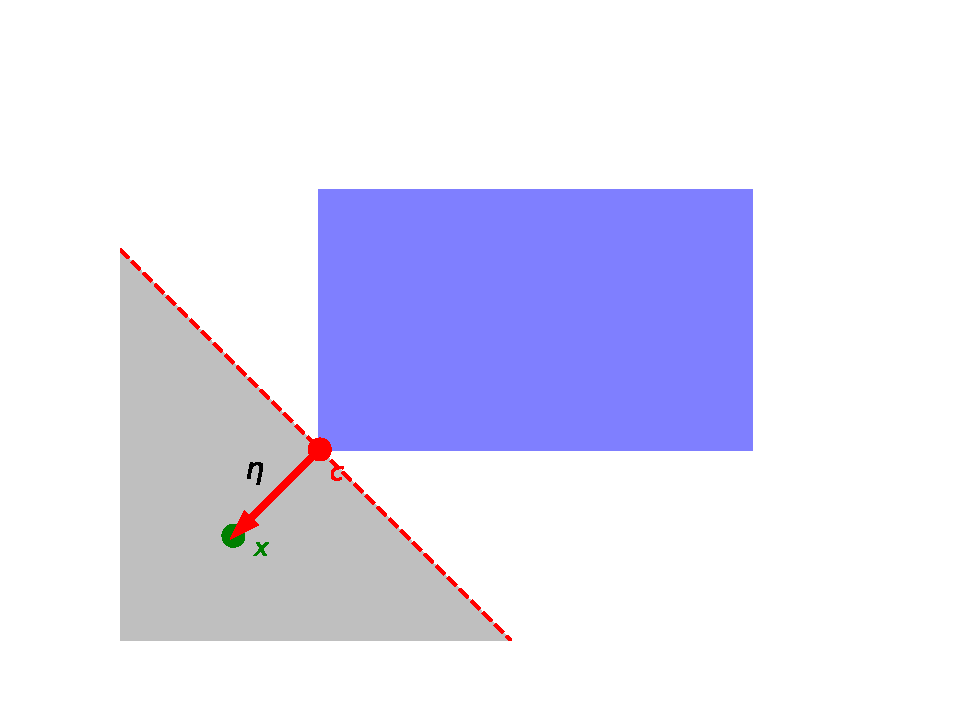
\includegraphics[width=0.75\linewidth]{figures//MPC/example_lcbf.pdf}
    \caption{In this figure, the CoM is represented as a green point, and the obstacle is a blue rectangle. The point on the obstacle's boundary that is closest to $\vec{x}$ is the red one, which represents $c$. The red vector connecting $c$ to $\vec{x}$ is $\eta$. The safe region defined by this LDCBF is the gray area. In that half-plane, the humanoid's CoM is free to move without hitting any obstacle.}
    \label{fig:example_LDCBF}
\end{figure}

If multiple obstacles are in the environment, the safe region is the intersection of the regions produced by each LDCBF.\\
By enforcing that the states $\mathbf{x}_{1...N+1}$ produced by the optimal inputs $\mathbf{u}_{0...N}$ computed by the MPC satisfy $h(\vec{x})>0$, we guarantee that, during the motion, the humanoid's CoM never collides with the obstacles.\\

Vectors $\eta$ and $c$ are computed as follows. Indicating with $A$ and $B$ the endpoints of the edge of the obstacle that is closest to $\vec{x}$ we have:
\begin{gather*}
    \overrightarrow{AX} \coloneqq \vec{x} - A, \qquad \overrightarrow{AB} \coloneqq B - A, \\
    t \coloneqq \frac{\overrightarrow{AX} \cdot \overrightarrow{AB}}{\left\lVert \overrightarrow{AB} \right\rVert ^2}, \qquad \tilde{t} = \max \left\{0,\; \min \left\{ 1,\; t\right\}\right\}, \\
    c \coloneqq A\, +\, \tilde{t}*\overrightarrow{AB}, \\
    \eta \coloneqq \left(-1\right)^{\xi} * \left( \vec{x} - c \right),
\end{gather*}

where $\xi=1$ if $\vec{x}$ is inside the obstacle, otherwise it is $0$.
Due to the presence of $\min$ and $\max$, the specified expressions of $c$ and $\eta$ are non-linear. However, the constraint enforced on the MPC solution at simulation time $k$ is based on the values of $c$ and $\eta$ computed at the beginning of the time step. Therefore, they are included in the constraint as constants, and the LDCBF becomes a linear combination of $\vec{x}$.

\subsubsection{Our variation of the LDCBF}
From Figure (\ref{fig:example_LDCBF}) it is evident that a such defined LDCBF constraint allows the humanoid to get very close to the obstacle's boundary. And, even though the CoM will not collide with it, the footstep positions provided by the MPC will likely overlap with the obstacle. Therefore, we developed a variant of the LDCBF proposed by Peng et al., defined as follows:

\begin{equation} \label{eq:ldcbf_variant}
h\left(\vec{x}\right) = \eta^T \left(\vec{x} - c\right) - \delta \geq 0,
\end{equation}

where $c$ and $\eta$ are the previously defined vectors, while $\delta$ is the distance that the CoM must keep from $c$ (i.e., from the obstacle's boundary) to satisfy the constraint. The result is shown in Figure \ref{fig:example_LDCBF_variant}\\
Forcing the control barrier function not to take values below a threshold allows us to take into account the footstep positions, and to generate trajectories that are not only feasible for the CoM, but for the motion of the whole humanoid.

\begin{figure}[h]
    \centering
    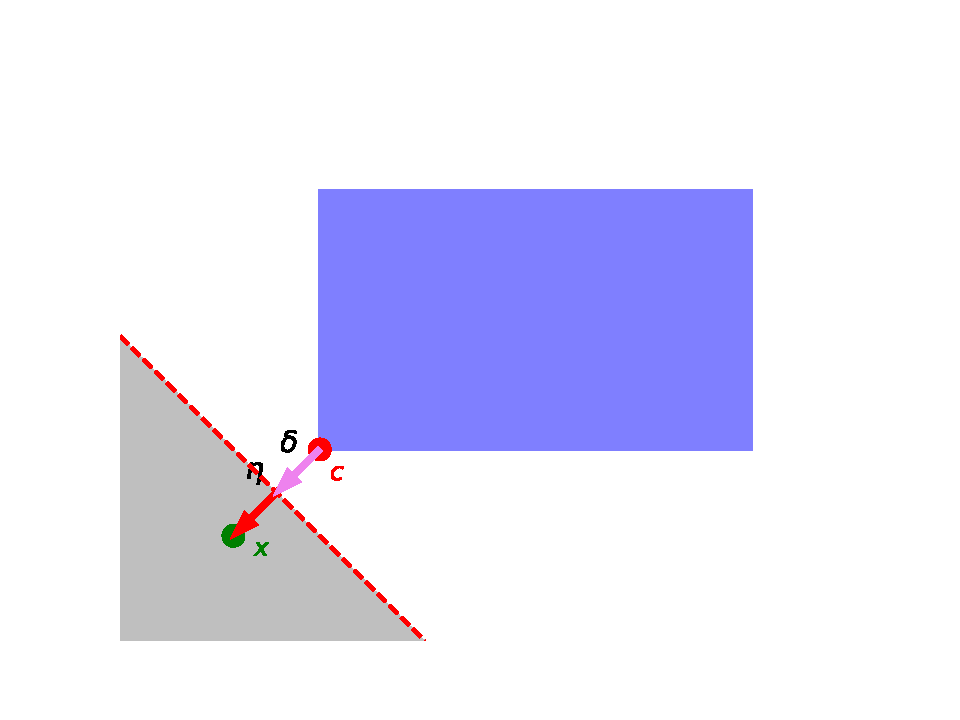
\includegraphics[width=0.75\linewidth]{figures//MPC/example_ldcbf_variant.pdf}
    \caption{This plot shows the same environment of Figure \ref{fig:example_LDCBF}, but here expression (\ref{eq:ldcbf_variant}) with $\delta > 0$ was used as LDCBF. It is clear that the safe zone is not adjacent to the obstacle, and $\vec{x}$ maintains a distance $\delta$ from the obstacle.}
    \label{fig:example_LDCBF_variant}
\end{figure}